\subsection{Steel beams}

\begin{figure}
  \begin{center}
  \includegraphics[width=120mm]{figures/steel_beams_key_plan}
  \end{center}
  \caption{Second floor beams key plan.}\label{fg_2nd_floor_beams_key_plan}
\end{figure}

\subsubsection{Steel beam at courtyard facade}
Continuous beam supporting the second floor trusses between the axes 1, 2 and 3 (see figure \ref{fg_2nd_floor_beams_key_plan}). The beam has two equal spans; L= 8.31 m ($27' - 3''$).

\paragraph{Design loads.}
The design loads are show in table \ref{tb_CD_reactions}. The beam then carries a the following loads:\\
\begin{itemize}
\item Dead load: $14.88\ kN/m$.
\item Live load: $22.86\ kN/m$.
\item Snow load: $10.05\ kN/m$.
\item Wind load: $-6.35\ kN/m$.
\end{itemize}

\begin{table}
  \begin{center}
  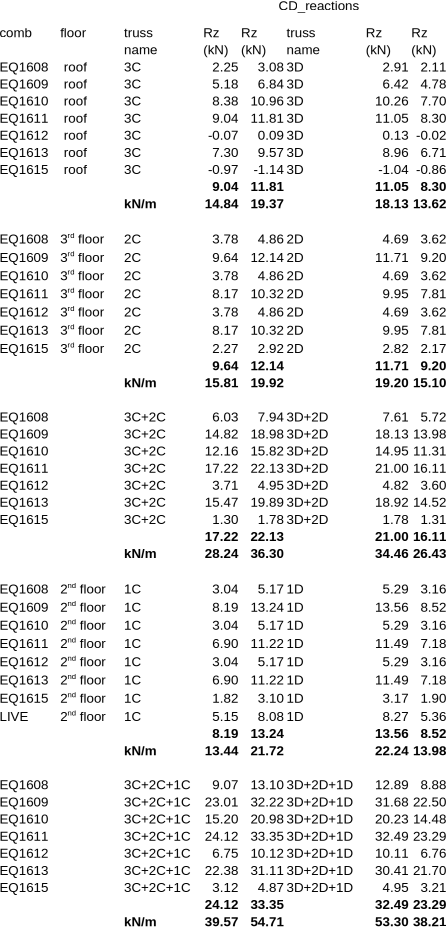
\includegraphics[width=75mm]{figures/CD_reactions}
  \end{center}
  \caption{Steel beam at courtyard facade.Trusses reactions.}\label{tb_CD_reactions}
\end{table}

\paragraph{Load combinations}

\subparagraph{Serviceability limit states}
\begin{center}
  \begin{tabular}{|l|l|}
    \hline
    SLS01 & $1.0 \times LL$ \\
    SLS02 & $1.0 \times DL+1.0 \times LL$ \\
    SLS03 & $1.0 \times DL+1.0 \times S$ \\
    \hline
  \end{tabular}
  \end{center}

\subparagraph{Ultimate limit states}
\begin{center}
  \begin{tabular}{|l|l|}
    \hline
ULS01 & $1.4 \times DL$ \\
ULS02 & $1.2 \times DL + 1.6 \times LL + 0.5 \times S$ \\
ULS03 & $1.2 \times DL + 1.6 \times S + 0.5 \times LL $ \\
ULS04 & $1.2 \times DL + 1.6 \times S + 0.5 \times W$ \\
ULS05 & $1.2 \times DL + 1.0 \times W + 0.5 \times LL $ \\
ULS06 & $1.2 \times DL + 0.5 \times LL + 0.2 \times S$ \\
ULS07 & $0.9 \times DL + 1.0 \times W$ \\
    \hline
  \end{tabular}
  \end{center}


\paragraph{Structural design of the beam.}

\subparagraph{Internal forces.}

\noindent Maximum induced moment:
\begin{equation}
  M_{max}= -513\ kN \cdot m
\end{equation}

\begin{figure}
\begin{center}
  \includegraphics[width= 90mm]{figures/courtyard_facade_beam_uls02_mz.png}
\end{center}
\caption{Courtyard facade steel beam. ULS02. $M_z$}
\end{figure}
  
\noindent Maximum induced shear:

\begin{equation}
  V_{max}= 309\ kN
\end{equation}

\begin{figure}
\begin{center}
  \includegraphics[width= 90mm]{figures/courtyard_facade_beam_uls02_vy.png}
\end{center}
\caption{Courtyard facade steel beam. ULS02. $V_y$}
\end{figure}

\subparagraph{W12X87 shape mechanical properties.} Steel: A572

\noindent Shear strength:
\begin{equation}
  V_u= 862.32\ kN 
\end{equation}
\noindent Structural shear check: $V_u = 862.32 > 309.00 = V_{max} \implies OK$

\noindent Resisting moment:
\begin{equation}
  M_u= 670.68\ kN\cdot m
\end{equation}

\noindent Structural bending check: $M_U = 670.68 > 513.00 = M_{max} \implies OK$

\subparagraph{Bending stiffness.}
The deflections obtained for SLS01, SLS02 and SLS03 are:

\begin{align}
  \Delta_{TL} &= 9.54\ mm < 15.38\ mm = \frac{L}{540} \implies OK\\
  \Delta_{TL} &= 10.40\ mm < 23.07\ mm = \frac{L}{360} \implies OK\\
  \Delta_{TL} &= 15.74\ mm < 23.07\ mm = \frac{L}{360} \implies OK
\end{align}

\subsubsection{Steel beam at corridor}
This beam supports the second floor trusses near the elevator well (see figure \ref{fg_2nd_floor_beams_key_plan}) . It has a main span of 6.91 m long ($22' - 8''$)  and a cantilever that spans 1.04 m ($3'-4''$).

\paragraph{Design loads.}
The design loads are shown in table \ref{tb_E_reactions}. The beam then carries a load of $31.66\ kN$ each $0.6 m (24'')$. 

\begin{table}
  \begin{center}
  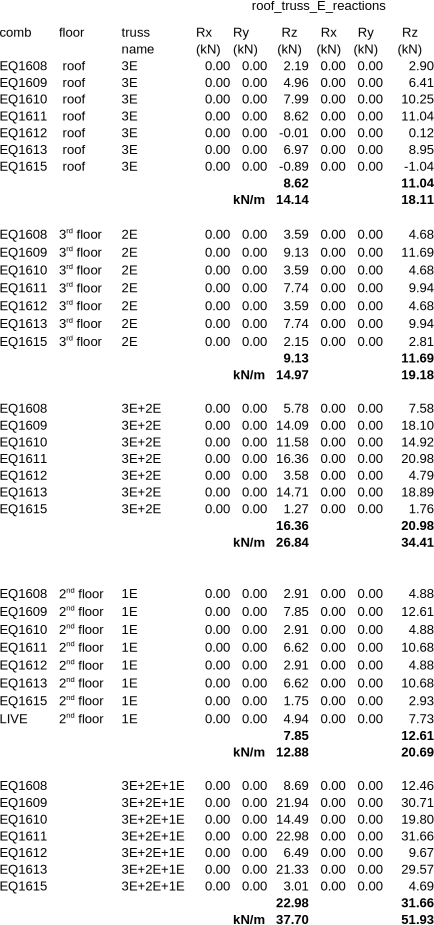
\includegraphics[width=75mm]{figures/E_reactions}
  \end{center}
  \caption{Steel beam at corridor. Trusses reactions.}\label{tb_E_reactions}
\end{table}

\paragraph{Structural design of the beam.}

\subparagraph{Loads.}

\begin{equation}
  w_{load}= 51.94\ kN/m
\end{equation}

\subparagraph{Internal forces.}

\noindent Maximum induced moment:

\begin{equation}
  M_{max}= 315.06\ kN m
\end{equation}

\noindent Maximum induced shear:

\begin{equation}
  V_{max}= 182.52\ kN
\end{equation}

\subparagraph{Structural shape (W21X50) mechanical properties.}
Steel: ASTM A-572

\noindent Shear strength:
\begin{equation}
  V_u= 607.72\ kN 
\end{equation}
\noindent Structural shear check: $V_u = 607.72 > 182.52 = V_{max} \implies OK$

\noindent Resisting moment:
\begin{equation}
  M_u= 371.86\ kN\cdot m
\end{equation}

\noindent Structural bending check: $M_U = 371.86 > 316.06 = M_{max} \implies OK$

\subparagraph{Bending stiffness.}
The deflection obtained is:

\begin{equation}
  \Delta_{TL}=16.88\ mm= \frac{L}{409} < \frac{span}{360} \implies OK
\end{equation}

\subsubsection{North steel beam}
This beam supports the second floor trusses near the stairs well at north facade (see figure \ref{fg_2nd_floor_beams_key_plan}) . It spans 7.26 m (~$23' - 10''$).

\paragraph{Design loads.}
The design loads are shown in table \ref{tb_E_reactions}.  The beam then carries a the following loads:\\
\begin{itemize}
\item Dead load: $15.52\ kN/m$.
\item Live load: $21.74\ kN/m$.
\item Snow load: $9.52\ kN/m$.
\item Wind load: $-6.01\ kN/m$.
\end{itemize}

\paragraph{Load combinations}

\subparagraph{Serviceability limit states}
\begin{center}
  \begin{tabular}{|l|l|}
    \hline
    SLS01 & $1.0 \times LL$ \\
    SLS02 & $1.0 \times DL+1.0 \times LL$ \\
    SLS03 & $1.0 \times DL+1.0 \times S$ \\
    \hline
  \end{tabular}
  \end{center}

\subparagraph{Ultimate limit states}
\begin{center}
  \begin{tabular}{|l|l|}
    \hline
ULS01 & $1.4 \times DL$ \\
ULS02 & $1.2 \times DL + 1.6 \times LL + 0.5 \times S$ \\
ULS03 & $1.2 \times DL + 1.6 \times S + 0.5 \times LL $ \\
ULS04 & $1.2 \times DL + 1.6 \times S + 0.5 \times W$ \\
ULS05 & $1.2 \times DL + 1.0 \times W + 0.5 \times LL $ \\
ULS06 & $1.2 \times DL + 0.5 \times LL + 0.2 \times S$ \\
ULS07 & $0.9 \times DL + 1.0 \times W$ \\
    \hline
  \end{tabular}
  \end{center}

\paragraph{Structural design of the beam.}

\subparagraph{Internal forces.}

\noindent Maximum induced moment:
\begin{equation}
  M_{max}= 383\ kN \cdot m
\end{equation}

\noindent Maximum induced shear:

\begin{equation}
  V_{max}= 211\ kN
\end{equation}

\subparagraph{W12X87 shape mechanical properties.} Steel: A572

\noindent Shear strength:
\begin{equation}
  V_u= 862.32\ kN 
\end{equation}
\noindent Structural shear check: $V_u = 862.32 > 211.00 = V_{max} \implies OK$

\noindent Resisting moment:
\begin{equation}
  M_u= 670.68\ kN\cdot m
\end{equation}

\noindent Structural bending check: $M_U = 670.68 > 383.00 = M_{max} \implies OK$

\subparagraph{Bending stiffness.}
The deflections obtained for SLS01, SLS02 and SLS03 are:

\begin{align}
  \Delta_{TL} &= 12.77\ mm < 13.45\ mm = \frac{L}{540} \implies OK\\
  \Delta_{TL} &= 14.71\ mm < 30.26\ mm = \frac{L}{240} \implies OK\\
  \Delta_{TL} &= 21.89\ mm < 30.26\ mm = \frac{L}{240} \implies OK
\end{align}
